\begin{answer}
\begin{figure}[H]
    \centering
    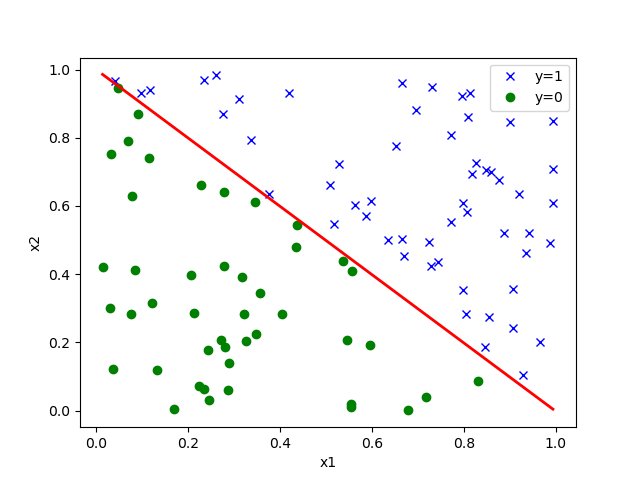
\includegraphics[width=0.5\linewidth]{ps2::q3::(b).png}
    \caption{ps2::q3::(b)}
    \label{fig:enter-label}
\end{figure}

Q1 What is the most notable difference in training the logistic regression
model on datasets A and B? 

Train on dataset A converges while train on dataset B doesn't. During training on dataset b, as iteration goes, the loss is 0 (ignore the loss noise by adding $\epsilon$) and the absolute value of theta keeps growing. \\
\newline

Q2: Investigate why the training procedure behaves unexpectedly on dataset B, but not on A. 

The main reason is that classes in the dataset B can be perfectly separated, meaning there exists a line (more generally, hyper plane) that can achieve 0 training error. Then the training prefer to minimize $y - Pred$, meaning $\theta$ will keep growing \\
\newline

Q3: Provide hard evidence (in the form of math, code, plots, etc.)
to corroborate your hypothesis for the misbehavior. Remember, you should address why
your explanation does not apply to A

Loss function is defined as follows
\begin{equation*}
	J(\theta)
	= -\frac{1}{\nexp} \sum_{i=1}^\nexp \left(y^{(i)}\log(h_{\theta}(x^{(i)}))
		+  (1 - y^{(i)})\log(1 - h_{\theta}(x^{(i)}))\right),
\end{equation*}
If the training set can be perfectly separated by a hyper plane, then $J(\theta)$ will be close to zero. That means 
\begin{align}
    h_{\theta}(x^{(i)}) \approx 1 \text{ when } y^{(i)} = 1 \\
    h_{\theta}(x^{(i)}) \approx 0 \text{ when } y^{(i)} = 0 
\end{align}
If the model find a $\theta$ that incur almost 0 loss for the loss function defined above, then theoretically, for any given constant $C$, a hyper plane defined by $C \theta^\top x = 0$ will also lead to 0 loss. Logistic model prefer $C$ to be big number to minimize the loss function, logistic model will never converge and $C$ will keep growing


\end{answer}
